%%This is a very basic article template.
%%There is just one section and two subsections.
\documentclass[a4paper,12pt]{scrartcl}
\usepackage{polski}
\usepackage[utf8]{inputenc}
\usepackage[T1]{fontenc}
\usepackage{datetime}

\usepackage{listings}
\usepackage{graphicx, graphics, epsfig, geometry, pslatex}
\usepackage{amsmath, amssymb}
\usepackage{url}

\usepackage{array}
\usepackage{times}
\usepackage{fullpage}
\usepackage{caption}

\newcommand{\figsource}[1]{
\captionsetup{font={scriptsize, it}}
\caption*{Źródło: \url{#1}}
\captionsetup{font={normalsize}}
}

\newcommand{\f}{\texttt}
\newcommand{\mytitlea}{Peer-to-peer web objects}
\newcommand{\mytitleb}{cacheing proxy}
\newcommand{\me}{Tomasz Drwięga}
\newcommand{\s}{ }

\newcommand{\kesz}{cache}
\newcommand{\kesza}{cache'a}
\newcommand{\keszowi}{cache'owi}
\newcommand{\keszem}{cache'em}
\newcommand{\keszu}{cache'u}
\newcommand{\keszujace}{cache'ujące}
\newcommand{\keszujacego}{cache'ującego}
\newcommand{\keszujacym}{cache'ującym}
\newcommand{\keszowania}{cache'owania}

\lstset{numbers=left,
	numberstyle=\tiny,
	%basicstyle=\footnotesize,
	showstringspaces=false,
	basicstyle=\footnotesize,
	breaklines=true,
	captionpos=b,
	tabsize=3,
	stepnumber=60,
	firstnumber=1,
	}
%opening
\title{\mytitlea \mytitleb}
\author{\me}

\makeindex

\begin{document}

% \parindent0pt
\pagestyle{empty}

\begin{titlepage}
\vspace*{\fill}
\begin{center}
\begin{picture}(300,510)
	\put( 0,520){\makebox(0,0)[l]{\large \bf \textsc{Wydział Podstawowych
	Problemów Techniki}}}
	\put( 0,500){\makebox(0,0)[l]{\large \bf \textsc{Politechniki Wrocławskiej}}}
	\put(15,280){\makebox(0,0)[l]{\Huge  \bf \textsc{\mytitlea}}}
	\put(80,250){\makebox(0,0)[l]{\Huge  \bf \textsc{\mytitleb}}}
	\put(95,220){\makebox(0,0)[l]{\Large     \textsc{\me}}}
	
	\put(190, 80){\makebox(0,0)[l]{\large  {Praca magisterska napisana}}}
	\put(190, 60){\makebox(0,0)[l]{\large  {pod kierunkiem}}}
	\put(190, 40){\makebox(0,0)[l]{\large  {dra Mirosława Korzeniowskiego}}}
	
	\put(110,-80){\makebox(0,0)[bl]{\large \bf \textsc{Wrocław 2013}}}
\end{picture}
\end{center}
\vspace*{\fill}
\end{titlepage}

\tableofcontents

\newpage

\pagestyle{headings}

\section*{Wstęp}

\subsection{Sformułowanie problemu}

\subsection{Istniejące rozwiązania}

\section{Historia keszowania}
Wraz z rosnącą liczbą użytkowników Internetu w latach dziewięćdziesiątych zaczęły pojawiać się problemy z dostępem do pewnych zasobów.
Duża liczba odwołań do popularnych strony, w krótkim czasie powodowała znaczące obciążenie serwerów, które dany zasób posiadały.
Czasami z powodu nadmiernego zalania\footnote{ang. \textit{flooded}, \textit{swamped}} żądaniami serwer nie był w stanie obsłużyć wszystkich przez co strona stawała się niedostępna.

\subsection{Serwery \keszujace}\label{sect_cache}
Jako rozwiązanie problemu ``gorących punktów'' (ang. \textit{hot spots}) pojawiły się serwery \keszujace. Rysunek \ref{fig_cache_server} przedstawia wprowadzenie transparentnego, lokalnego \kesza\s i jego relację z serwerem docelowym. 
Żądania zasobów wychodzące od użytkowników końcowych są w pierwszej kolejności obsługiwane przez serwer \keszujace, który odpowiada zapamiętanym zasobem lub kontaktuje się z serwerem docelowym i zapamiętuje odpowiedź.

\begin{figure}[ht]
\centering
\includegraphics[width=0.9\linewidth]{img/media_server2_edge.jpg}
\figsource{http://www.neatfilm.com/2005/11/16/distributed-media-server-infrastructure/}
\caption{
Przykład lokalnego serwera \keszujacego.
Zamiast wielokrotnie odwoływać się do docelowego serwera, który zawiera daną stronę
możemy zapamiętać ją na serwerze \keszujacym. Takie rozwiązanie niesie ze sobą zalety
zarówno dla administratorów serwera w Chicago, jak i użytkowników sieci w Japoni:
mniej żądąń skutkuje mniejszym obciążeniem serwera, a ``lokalność'' serwera \keszujacego\s zmniejsza opóźnienia i zwiększa szybkość transferu zasobu.
}
\label{fig_cache_server}
\end{figure}

Wprowadzenie \keszowania\s niesie ze sobą szereg zalet nie tylko dla administratorówserwerów zawierających zasoby. Serwery znajdujące się na granicy sieci lokalnej z Internetem (jak na rysunku \ref{fig_cache_server}) oferują użytkownikom tej sieci lepszy transfer i mniejsze opóźnienia w dostępie do popularnych zasobów.
Ponieważ łącze wychodzące z sieci ma ograniczoną przepustowość, \kesz\s pozwala również na oszczędniejsze wykorzystanie łącza, a tym samym poprawę jakości dostępu do Internetu.

\subsection{Rozproszony \kesz}
Rozwiązanie przedstawione w rozdziale \ref{sect_cache} pozwala na odciążenie serwera docelowego. Zastanówmy się jednak co będzie się działo w przypadku zwiększania liczby użytkowników korzystających z serwera \keszujacego. Duża liczba żądań może spowodować dokładnie taką samą sytuację jak w przypadku serwera docelowego - \kesz\s zostanie zalany i nie będzie w stanie obsłużyć wszystkich zapytań.

W ramach projektu Harvest \cite{bowman1994harvest} A. Chankhunthod i inni \cite{chankhunthod1995hierarchical} opracowali \kesz\s hierarchiczny.


\begin{figure}[h]
\centering
\includegraphics[width=0.9\linewidth]{img/hierarchical.jpg}
\label{fig_cache_hierarchical}
\figsource{http://www.cse.wustl.edu/~jain/cis788-99/ftp/web_caching/}
\caption{Połączenie kilu serwerów \keszujacych\s w system hierarchiczny. Każdy z serwerów znajdujących się w liściach obsługuje określoną liczbę użytkowników. Zapytania o zasoby, które nie znajdują się w \keszu\s wysyłane są do rodzica.}
\end{figure}



\section{Opis działania}

\section{Analiza bezpieczeństwa i wydajności}
\subsection{System, w którym klucz == url}
Można śledzić co przeglądają użytkownicy.

Nie jest wymagane STORE zasobu - węzły mogą rozpocząć pobieranie podczas operacji SEARCH.

\subsection{System, w którym klucz == hash(url)}
Dodatkowo zawartość plików może być szyfrowana prawdziwym \f{url}.
W ten sposób nie można podglądać zawartości plików. 

\section{Analiza różnych metod cachowania}
Cache wielopoziomowy:
\begin{enumerate}
  \item w pamięci,
  \item na dysku,
  \item w sieci P2P (te dane również w pamięci, na dysku)
\end{enumerate}
Różne strategie przechodzenia między poziomami.

\section{Testy}
\subsection{Spreparowane dane}

\subsection{Wdrożenie}

\section{Implementaja}
\subsection{Wybór technologii}
Tutaj próby zrobienia tego w JS jako plugin do przeglądarki.
\subsection{Biblioteki}
Twisted, Entangled.
\subsection{Instalacja i uruchomienie}


\bibliographystyle{plain}

\bibliography{document}

\end{document}

